\documentclass[sigconf,nonacm]{acmart}

% --- course report: drop the ACM publication boilerplate ---
\settopmatter{printacmref=false}
\setcopyright{rightsretained}
\renewcommand\footnotetextcopyrightpermission[1]{}
\pagestyle{plain}

\usepackage{amsmath}
\usepackage{amssymb}
\usepackage{subcaption}
\setlength{\emergencystretch}{1.5em}

% The figures in figures/ and the table bodies in tables/ are generated from the stored
% measurements by code/experiments/5_comparison/paper_assets.py (see README.md). Numbers in the
% running text are recomputed by text_numbers.py and count_outcomes.py in the same directory.
\newcommand{\ProverGPU}{RTX 2080~Ti}
\newcommand{\VerifierCPU}{Intel Xeon Silver 4114}
\newcommand{\VerifierThreads}{8}
\newcommand{\LLMNote}{ ($^\ast$extrapolated from 1- and 2-block builds)}


\newcommand{\T}{\top}
\newcommand{\F}{\mathbb{F}_p}
\newcommand{\enc}{\mathrm{Enc}}
\newcommand{\Kpre}{\mathsf{K}_{\mathrm{pre}}}
\newcommand{\sC}{\mathsf{C}}
\newcommand{\sK}{\mathsf{K}}
\newcommand{\para}[1]{\smallskip\noindent\textbf{#1}\quad}

\begin{document}

\title{Certified but Compromised: Breaking and Fixing\\ Lightweight Proofs of Inference}
\subtitle{Final Report --- Trustworthy Machine Learning, Spring 2026}

\author{Ofek Lavi}
\affiliation{\institution{Tel Aviv University}\city{Tel Aviv}\country{Israel}}
\email{ofeklavi@mail.tau.ac.il}

\author{Erel Barzilay}
\affiliation{\institution{Tel Aviv University}\city{Tel Aviv}\country{Israel}}
\email{erelbarzilay@mail.tau.ac.il}

\author{Edo Kadosh}
\affiliation{\institution{Tel Aviv University}\city{Tel Aviv}\country{Israel}}
\email{edo@mail.tau.ac.il}

\begin{abstract}
When a large model runs in the cloud, its users cannot tell whether an answer came from the
agreed weights. zkSNARK proofs of inference settle this but take minutes per query on large
models, so Anchuri et al.\ (SaTML~2026) proposed a lightweight alternative in which the client
re-checks one random path through a committed computation. Its guarantee covers a provider that
runs some other model. We show that a provider that runs the committed model but changes a
single neuron is accepted 99.8\% of the time on an MNIST network. Applied only to triggered
inputs, the edit is a backdoor that leaves the committed weights clean, and on the real OPT-6.7B
one neuron changes the next token of every prompt we tried. Against an adversary who knows the
sampler, no rule that ignores the claimed values does better than uniform sampling, and the best
rule we found that uses them has a blind spot. Our defence checks every layer with one random
linear combination (Freivalds' check), in exact integer arithmetic, against a
Reed--Solomon/Merkle commitment to the weights, and accepts a wrong output with probability at
most $2^{-\lambda}$ without a trusted setup. It rejected all 2{,}895 attacks, on models from
LeNet-5 to Llama-2-13B and on truncated builds of larger ones. Its prover is one to four
orders of magnitude faster than published zkSNARK provers, and 157$\times$ faster than zkLLM's
own code on our GPU for Llama-2-7B. With optimisations that keep the bound, it also verifies
faster and sends less, non-interactively, than zkCNN on LeNet-5 and, for GPT-2's next-token
logits, than DeepProve's transparent configuration. Its remaining cost is a proof that grows
with the activations.
\end{abstract}

\keywords{verifiable inference, proof of inference, integrity attacks, Freivalds' algorithm, zkML}

\maketitle

% =====================================================================================
\section{Introduction}

\begin{figure*}[t]
  \centering
  \begin{subfigure}[b]{0.31\textwidth}
    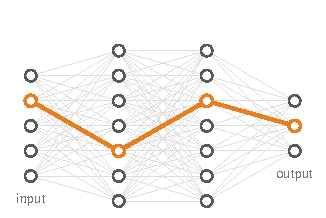
\includegraphics[width=\linewidth]{figures/overview_path.pdf}
    \caption{Path test: one node per layer}
    \label{fig:overview-path}
  \end{subfigure}\hfill
  \begin{subfigure}[b]{0.31\textwidth}
    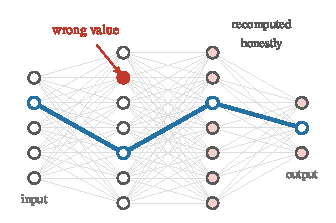
\includegraphics[width=\linewidth]{figures/overview_attack.pdf}
    \caption{Attack: caught with prob.\ $1/N$}
    \label{fig:overview-attack}
  \end{subfigure}\hfill
  \begin{subfigure}[b]{0.31\textwidth}
    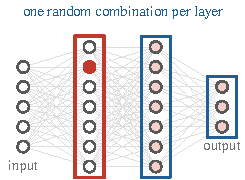
\includegraphics[width=\linewidth]{figures/overview_defence.pdf}
    \caption{Defence: caught with prob.\ $1-2^{-\lambda}$}
    \label{fig:overview-defence}
  \end{subfigure}
  \Description{Three small network diagrams: a random path checked by the path protocol, a
  single tampered neuron that the path misses, and every layer checked by our defence.}
  \caption{A single tampered neuron, with everything after it recomputed honestly, leaves one
  inconsistent node: a random path rarely visits it (b), while one random combination per layer
  catches it (c).}
  \label{fig:overview}
\end{figure*}

Consider a company that pays a cloud provider to serve a licensed or fine-tuned language model to
its users. Nothing in a response shows that the provider ran that model with the agreed weights
rather than a cheaper quantised copy, a model with a few edited weights, or one that misbehaves
on certain inputs. The company cannot re-run the model to find out, since it lacks the weights
and the hardware; that is why it outsourced inference. A \emph{proof of inference} closes this
gap. With each answer the provider sends a proof, and the client runs a check, much cheaper than
inference, that fails with high probability unless the answer was computed with the agreed
weights on this input.

zkSNARKs~\cite{zkcnn,zkml,zkllm,zkgpt,deepprove} prove that the answer is correct and can keep
the weights secret. Their proofs are usually small and fast to check, but producing one takes far
longer than inference; zkLLM needs
about ten minutes on an A100 for one Llama-2-7B prompt~\cite{zkllm}. Anchuri et
al.~\cite{anchuri2026verifiable} proposed a much lighter approach. The provider commits to the
full execution trace with a Merkle tree, and the client checks the computation along \emph{one
random path} from an output neuron back to the input, against a commitment to the weights.
Proving drops from minutes to milliseconds. A different model produces a trace that differs from
the correct one in many places, so a random path is likely to hit one of them, and Anchuri et
al.\ accordingly prove \emph{other-model} soundness, against a provider that honestly runs some
different model. They note that one path cannot catch a single changed node with probability
above $1/N$ in a layer of width $N$, and they leave full soundness for LLMs open.

\para{What we did.} We reimplemented the protocol (no code was released), reproduced its main
claims, and asked what a provider can do if it keeps the committed model and changes only what it
needs to. It can overwrite \emph{a single neuron} and recompute everything after it honestly
(Figures~\ref{fig:overview-path} and~\ref{fig:overview-attack}). The trace is then inconsistent at
one node, which a random path visits with probability $1/N$, so almost every tampered answer is
accepted. Applied only to inputs that carry a trigger, the edit is a backdoor in the serving
code, which leaves the committed weights clean and answers clean queries bit for bit as before. The
attack carries over to a real 6.7B-parameter model. Auditing does not close the gap, because the
provider chooses which queries to tamper with, and tampering with $k$ of them is caught with
probability at most $k/N$. Nor does sampling more paths, or sampling adaptively, as Anchuri et
al.\ suggest. Uniform sampling is already optimal among rules that ignore the claimed values, the
best rule we found that uses them has a blind spot, and reaching $2^{-40}$ forces the path
protocol to open essentially the whole model and trace.

This led us to a different design (Figure~\ref{fig:overview-defence}). The verifier tests one
random linear combination of all the neurons of every layer (Freivalds'
algorithm~\cite{freivalds1977}). When it does not hold the weights, it checks the combination
against a Reed--Solomon-encoded, Merkle-committed copy of them in the style of
Ligero~\cite{ligero}, so it still stores 32 bytes per weight matrix. The model runs as an int8
network whose results are bit-identical on the provider's GPU and on the client, which makes the
test exact. A tampered value anywhere in the network is then caught with probability
$1-2^{-\lambda}$ instead of $1/N$, and the prover's extra work grows with the model but not with
the input. At equal or higher security our proofs are also the smaller ones: catching the
single-neuron attack on a 64-token Llama-2-7B prompt with probability $1-2^{-40}$ takes paths that
open about 13.7\,GB, while our proof at $2^{-128}$ is 762\,MB, or 329\,MB after the optimisations
of Section~\ref{sec:opt}.
Spot-checking a few neurons exactly leaves the rest of the network unconstrained; one random
combination per layer constrains all of it.

\para{Contributions.}
\begin{itemize}
  \item \textbf{An attack} that exploits the $1/N$ limit acknowledged in~\cite{anchuri2026verifiable}.
  One tampered neuron is accepted with probability $1-1/N$ (99.6--99.8\% on MNIST), works as a
  trigger backdoor that leaves the weights and clean answers unchanged, and changes the next token
  of 40 of 40 prompts on the real OPT-6.7B.
  \item \textbf{A bound on sampling-based fixes:} no value-blind sampler beats uniform sampling,
  the contribution-weighted sampler is blind to zeroed neurons, and $2^{-40}$ requires opening
  essentially the whole model and trace.
  \item \textbf{A full-soundness protocol} for whole CNNs and transformers, with error
  $2^{-\lambda}$ and no trusted setup, and optimisations that keep the bound and shrink the
  committed-weights proof 2.0--4.2$\times$ for images and prompts of up to 512 tokens.
  \item \textbf{A same-architecture evaluation} on 6 image classifiers and 10 LLM architectures
  up to 13B parameters, against~\cite{anchuri2026verifiable}, 17 published systems and zkLLM's
  code on our GPU. On matched models our prover is 53--32{,}000$\times$ faster than the zkSNARK
  provers, and on
  LeNet-5 and on GPT-2's next-token logits the optimised protocol beats zkCNN and DeepProve's
  transparent configuration on all three costs (prover time, verifier time and proof size). Code
  and raw measurements are released.
\end{itemize}

% =====================================================================================
\section{Related Work}

\para{zkSNARK proofs of inference.} A long line of work compiles neural networks into
zero-knowledge proofs. For CNNs these include sum-check/GKR provers~\cite{gkr} such as
zkCNN~\cite{zkcnn} and zkPyTorch~\cite{zkpytorch}, and pairing- or Plonk-based systems such as
vCNN~\cite{vcnn}, ZEN~\cite{zen}, ZENO~\cite{zeno}, ZKML~\cite{zkml}, EZKL~\cite{ezkl} and
Bionetta~\cite{bionetta}; Mystique~\cite{mystique} is an interactive, VOLE-based alternative.
For LLMs they include zkLLM~\cite{zkllm} (also interactive), zkGPT~\cite{zkgpt},
DeepProve~\cite{deepprove}, ZKTorch~\cite{zktorch} and Jolt Atlas~\cite{joltatlas}. They give
computational soundness and mostly small proofs, but their provers are far slower than
inference: from half a second for LeNet-5 to minutes or hours for larger models.

\para{Freivalds-style checks.} SafetyNets~\cite{safetynets} uses interactive proofs for networks
with quadratic activations. Slalom~\cite{slalom} checks every linear layer of a GPU computation
from inside an SGX enclave with Freivalds' algorithm, in exact arithmetic modulo a 24-bit prime
and optionally with a precomputed secret challenge; TwinShield~\cite{twinshield} and
VeriAttn~\cite{veriattn} extend this to attention inside TEEs. Two recent works need no
enclave. Maverick~\cite{maverick} combines sparse Freivalds checks with a linear code, for a
client that knows the weights and draws a fresh challenge per query. LAMP~\cite{lamp} lets a
verifier that holds only a commitment check one matrix product, using Freivalds' check and
Reed--Solomon proximity testing inside a Groth16 SNARK.

\para{Sampling, fingerprints and optimistic protocols.} Anchuri et
al.~\cite{anchuri2026verifiable} spot-check random paths and argue security through trace
separation; SLP~\cite{slp} samples which layers receive a SNARK. TOPLOC~\cite{toploc} and
SVIP~\cite{svip} fingerprint hidden states, with empirical guarantees. Verde~\cite{verde},
opML~\cite{opml} and TAO~\cite{tao} resolve disputes and assume an honest party or an active
challenger.

\para{Where we fit.} To our knowledge, ours is the first protocol with full soundness
$2^{-\lambda}$ in the setting of~\cite{anchuri2026verifiable}, a client holding a 32-byte
commitment per weight matrix, for complete CNNs and transformers without a SNARK, a TEE or a
structured reference string. Its parts are known: Freivalds' check, exact integer arithmetic and
client-side non-linear layers (Slalom, Maverick), and a Reed--Solomon-encoded Merkle commitment
opened at random columns (Ligero, LAMP). We contribute the attack, the bound on sampling, their
composition into a layer-chained protocol with an end-to-end soundness proof, optimisations that
keep that bound, and a same-architecture comparison.

% =====================================================================================
\section{Breaking Path Sampling}

\subsection{Setting and threat model}
A model $M$ has a public architecture and secret or public weights. The provider acts as the
prover and the client as the verifier. Before any query the client obtains a commitment $C_M$ to
the weights, for example from the model owner. As in~\cite{anchuri2026verifiable}, we assume
that $C_M$ is computed honestly; unlike a SNARK's trusted setup it involves no secret randomness,
and anyone who holds the weights can recompute it. For each query $x$ the provider returns a
claimed output $y$ and a proof, and may deviate from the protocol arbitrarily. We require
\emph{completeness} (honest answers are always accepted) and \emph{full soundness}: any
$y \neq M(x)$ is rejected except with probability $\varepsilon$. Anchuri et al.\ prove only
\emph{other-model soundness}, in which the adversary must honestly run some different model. We
consider three trust settings. In $\sC$ the client holds only $C_M$ (32 bytes per weight matrix),
as in~\cite{anchuri2026verifiable} and the zkSNARKs; in $\sK$ it knows the weights; and $\Kpre$
is $\sK$ with a secret challenge precomputed once per model, as in Slalom's preprocessing mode.

\subsection{The path test and the single-neuron attack}
\label{sec:attack}
In the protocol of~\cite{anchuri2026verifiable} (RandPathTest) the prover commits to every
activation $a_j$ of the forward pass with a Merkle tree. The verifier chooses a random output
neuron and walks back to the input, moving to a random parent at each layer. At every node $j$ on
the path it opens the parents' activations and the weights $w_{ij}$ from $C_M$ and checks
$a_j = \phi\big(\sum_{i \in G_j} w_{ij} a_i\big)$, where $G_j$ is the set of parents of $j$ and
$\phi$ the activation. A path opens one weight row per layer, so the proof and the prover's work
stay small.

\para{The single-neuron attack.} Our adversary runs the correct model on $x$, picks one neuron
$j$, and replaces $a_j$ by a value that makes the output wrong (untargeted) or equal to a class of
its choice (targeted). It then recomputes all later layers \emph{with the true weights}. Every
later node is consistent with its parents and every earlier node is untouched, so $j$ is the only
node whose local check fails. The verifier notices the attack only if its path visits $j$, which
happens with probability $1/N$ in a layer of width $N$, or $1-(1-1/N)^s$ with $s$ paths. Applied
only to inputs that contain a trigger, the attack becomes a backdoor in the serving code. The
prover keeps the committed weights and answers clean queries bit for bit honestly, so no
inspection of the weights reveals it and the clean-accuracy gap is zero by construction.

\subsection{Why sampling cannot fix it}
Anchuri et al.\ suggest sampling more paths, or sampling where it matters instead of uniformly.
Against an adversary who knows the rule, neither helps if the rule ignores the claimed values.

\begin{theorem}[uniform sampling is minimax-optimal]
Fix a layer, let $U$ be the set of its neurons whose change can flip the output, and consider any
sampler that opens at most $s$ nodes of the layer, chosen independently of the claimed trace. Let
$\pi(v)$ be the probability that node $v$ is opened. Then $\min_{v\in U} \pi(v) \le s/|U|$, with
equality only if $\pi$ is uniform on $U$.
\end{theorem}

\noindent An adversary who knows the sampler tampers with a node of $U$ that minimises $\pi$, so
it is detected with probability at most $s/|U|$. The bound holds because a minimum is at most the
average and the $\pi(v)$ sum to at most $s$. Constant detection therefore needs $s=\Omega(|U|)$ openings per layer, linear in the
width, which is the cost the protocol was designed to avoid. Samplers that look at the claimed
values are not safe either. The most effective one we found steps to parent $i$ with probability
proportional to its contribution $|w_{ij} a_i|$, so it never visits a neuron whose claimed
activation is zero, and an adversary who flips the output by zeroing a few neurons is never
detected. A floor $\delta$, sampling by $|w_{ij}|(|a_i|+\delta)$, removes this blind spot but
leaves detection at a few percent (Section~\ref{sec:break}), and a forgery that keeps every value
within its neuron's natural range gives a range check nothing to flag.

\subsection{The attack in practice}
\label{sec:break}

\para{Reproduction.} Our implementation behaves as Anchuri et al.\ describe. On MNIST versions of
four of their substitute-model settings (three from their experiments, one from their motivation),
honest provers were accepted in all 3{,}000 runs of each. Substitute models were caught in
99.8--100\% of runs, including an 8-bit quantised copy that agrees with $M$ on all 150 evaluated
queries. Exact equality, by contrast, accepts an honest
prover in only 21--37\% of runs, because a layer-wide matrix product and a single-neuron dot
product round differently, so the prescribed tolerance of $10^{-4}$ is necessary for completeness.

\begin{table}[t]
  \caption{Attacks on the path protocol (one path). The forgeries of~\cite{anchuri2026verifiable}
  corrupt hundreds of the MLP's 778 trace nodes and are always caught; ours leave 1--14
  inconsistent nodes and are almost never caught.}
  \label{tab:attack}
  \small
  \begin{tabular}{lrr}
    \toprule
    Attack & inconsistent nodes & accepted \\
    \midrule
    \multicolumn{3}{l}{\emph{Forgeries of~\cite{anchuri2026verifiable}, MNIST MLP}} \\
    Substitute model $\tilde M$ & $\approx$574 & 0.000 \\
    Inverse transform & 591 & 0.000 \\
    Logit swap & 256 & 0.000 \\
    Gradient reconstruction & $\approx$778 & 0.000 \\
    \multicolumn{3}{l}{\emph{Our attacks, MNIST MLP}} \\
    Single neuron, layer 1 & 1 & \textbf{0.998} \\
    Single neuron, layer 2 & 1 & \textbf{0.996} \\
    Backdoor, triggered inputs & 1 & \textbf{0.998} \\
    Stealthy (in natural range) & $\approx$5 & \textbf{0.989} \\
    Zeroing vs.\ contribution sampler & $\approx$14 & \textbf{1.000} \\
    \multicolumn{3}{l}{\emph{Our attacks, OPT-6.7B (real weights)}} \\
    One FFN neuron (40/40 prompts) & 1 & \textbf{0.99994} \\
    Backdoor, target ``back'' (40/40) & 1 & \textbf{0.99994} \\
    \bottomrule
  \end{tabular}
\end{table}

\para{The single-neuron attack.} Table~\ref{tab:attack} gives the number of inconsistent trace
nodes and the exact acceptance probability, computed by dynamic programming over the paths. The
forgeries of~\cite{anchuri2026verifiable} (its substitute model, the inverse-transform and
logit-swap forgeries of its Appendices~E and~F, and the gradient reconstruction of its
Section~7.2) corrupt hundreds of nodes and are always caught. One tampered neuron is accepted
with the predicted probability $1-1/N$, and in 99.96\% of 2{,}300 end-to-end runs. Triggered by a
$3{\times}3$ bright patch, the backdoor returns the honest output on every clean query and
succeeds on every triggered query not already in the target class. Keeping each forged value
below its neuron's 95th percentile takes about five neurons and still passes 99\% of the time,
and with 250 paths the attack is still accepted 61\% of the time.

\para{Other samplers.} Against an adversary who knows the rule, uniform sampling detects 0.20\%
of attacks, a static importance score 0.11\%, and gradient saliency, which a verifier cannot
compute without the model, 0.016\%. Contribution weighting detects nothing: zeroing about 14 of
the 512 neurons flips the prediction, and end-to-end runs accepted 2{,}000 of 2{,}000 attacks.
Zero is also these neurons' most common value (65\% of inputs), so activation statistics do not
flag the attack. A floor $\delta=1$ raises detection to 2\% (10$\times$ uniform); other floors
give 0.9--6$\times$.

\para{Larger models.} On every CNN and every test query, changing one penultimate neuron suffices
to flip the prediction. One path catches it with probability 1/84 (LeNet-5) to 1/512, and the least-visited neuron with
probability as low as 1/28 million; $2^{-40}$ takes 2{,}316--14{,}182 paths, which open the whole
model and trace (Figure~\ref{fig:security}). On Llama-2-7B one path detects the attack with
probability 1/11{,}008, and $2^{-40}$ needs about 305{,}000 paths ($\approx$13.7\,GB with the fp16
weights of~\cite{anchuri2026verifiable}, at 64 tokens).

\para{A real LLM.} On the real OPT-6.7B (fp16), the attacker ranks a few FFN neurons of layers 8,
16, 24 and 31 at the last position, by gradient and by their direct effect on the logits, and
finds the smallest change to one of them that changes the next token. One neuron sufficed for
all 40 prompts. A fixed-target backdoor is more constrained, because the final LayerNorm makes each
neuron force only its own \emph{saturation token} as its activation grows: the last layer's
16{,}384 neurons reach 6{,}187 of the 50{,}272 tokens. The backdoor succeeds for a reachable
target (``\texttt{back}'': 40/40 triggered prompts, clean prompts unchanged) and fails for
``\texttt{hacked}'' (0/40). A per-neuron range check would flag its values, which exceed the
neurons' natural range, but the path protocol has none; one path detects the backdoor with
probability 1/16{,}384, and $2^{-40}$ needs 454{,}248 paths.

% =====================================================================================
\section{Checking Every Layer}
\label{sec:defence}

Our verifier tests one random linear combination of all the neurons of each weight layer. A wrong
value anywhere in the layer changes this combination except with probability $1/p$, so the test
needs no assumption about where the adversary tampers. We build it in four steps.

\subsection{Construction}

\para{Step 1: an exact integer model.} A random combination is a reliable test only if both sides
compute exactly the same numbers, so the model runs in integers. Following integer-only
inference~\cite{jacob2018quant}, each weight layer computes $Z = W X + b$, where $W$ is int8 with
one scale per output channel, $X$ is int8 with one scale per tensor, and BatchNorm is folded into
$W$ and $b$. The next layer's input is obtained by fixed-point requantisation followed by the
activation or pooling, and convolutions become matrix products through im2col. On the prover's
GPU the products are computed in float32 chunks of at most 1{,}024 terms, so every partial sum
stays below $2^{24}$ in magnitude and is exact, and the prover's results are bit-identical to the
verifier's. Exactness also removes the floating-point tolerance of the path protocol, which
leaves an attacker room to hide small changes.

\para{Step 2: only weight products need a proof.} For every weight layer $\ell$ the prover sends
the claimed pre-activations $Z_\ell$, the \emph{claims}. The verifier recomputes every operation
that does not involve the weights from the claims of earlier layers: requantisation, ReLU,
pooling, residual additions, LayerNorm/RMSNorm, GELU/SiLU (by table look-up), RoPE, softmax, and
the attention products $QK^\T$ and $PV$. Each weight layer's input $X_\ell$ is therefore the
verifier's own computation, and what remains is to check $Z_\ell = W_\ell X_\ell + b_\ell$ for
every $\ell$. Because each $X_\ell$ is derived from the claims of earlier layers, the checks are
chained, so a prover cannot pass one layer's check with one value and feed another into the next.

\para{Step 3: Freivalds' check.} Write $A_\ell = [W_\ell \,|\, b_\ell]$, a matrix with $N$ rows
(one per output neuron) and row length $k$, and let $T$ be the number of columns of $X_\ell$
(pixels or tokens); we drop the subscript $\ell$ from $N$, $k$ and $T$ when the layer is clear.
The verifier draws a random $\chi \in \F^{N}$ and checks
\begin{equation}
  \chi^\T Z_\ell \;=\; \underbrace{(\chi^\T A_\ell)}_{u_\ell}\,[X_\ell; \mathbf{1}] ,
  \label{eq:freivalds}
\end{equation}
where we call $u_\ell$ the \emph{folded row}. Let $D = Z_\ell - A_\ell [X_\ell; \mathbf{1}]$; the
two sides of~\eqref{eq:freivalds} differ by $\chi^\T D$. If $D_{im} \ne 0$, entry $m$ of
$\chi^\T D$ equals $\chi_i D_{im}$ plus terms that do not involve $\chi_i$, so exactly one value
of $\chi_i$ makes it vanish, and a wrong layer passes with probability at most $1/p$, or $p^{-r}$
with $r$ independent vectors. This holds however many values are wrong and wherever they are: a
single tampered neuron is caught as reliably as a wholly wrong layer. Both sides cost
$O((N+k)T)$, against $O(NkT)$ for recomputing the layer.

We work in the BabyBear field $\F$, $p = 15\cdot2^{27}+1 \approx 2^{31}$. Integers map into $\F$
without wrap-around as long as they are small, and both sides enforce this. The verifier
range-checks every claim ($|z| < 2^{29}$), and setup checks that every honest pre-activation is
in the same range ($128\sum_c |w_{ic}| + |b_i| < 2^{29}$ for every row $i$, since int8 inputs are
at most 128 in magnitude). A wrong claim and the correct value then differ by less than
$2^{30} < p$, so they remain distinct in $\F$.

\para{Step 4: committed weights.} In setting $\sC$ the verifier cannot compute $u_\ell$, so the
prover sends it. Opening $t$ random entries of $u_\ell$ against the weights would be weak: a
prover who changes one of the $k$ entries escapes with probability $1-t/k$. We therefore commit
to an \emph{encoded} copy of the weights, in the style of Ligero~\cite{ligero}. At setup every row
of $A_\ell$ is padded with zeros to a power of two $\bar k \ge k$ and Reed--Solomon
encoded~\cite{reedsolomon1960} to length $n_\ell$ ($4\bar k$ in the basic protocol), giving
$\hat A_\ell$, and $C_M$ holds one Merkle root~\cite{merkle1987} per weight matrix, over the
columns of $\hat A_\ell$. Encoding is linear, so $\chi^\T \hat A_\ell = \enc(\chi^\T A_\ell)$. The
verifier encodes the claimed $u_\ell$ itself, opens $t$ random columns $c$, and checks
$\chi^\T \hat A_{\ell,c} = \enc(u_\ell)_c$. If $u_\ell$ is wrong, $\enc(u_\ell)$ and
$\enc(\chi^\T A_\ell)$ are distinct codewords that agree on at most $k-1$ of the $n_\ell$
positions, so $t$ distinct columns all miss the difference with probability at most
$((k-1)/n_\ell)^t < 4^{-t}$.

\begin{figure}[t]
  \centering
  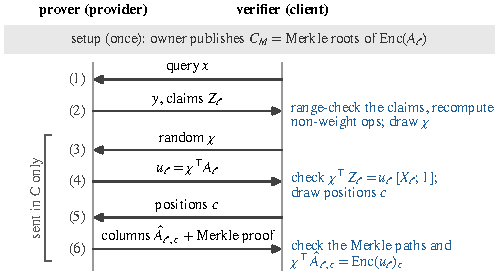
\includegraphics[width=\columnwidth]{figures/protocol.pdf}
  \Description{Message sequence between prover and verifier: query, output and claims, random
  challenge, folded rows, column positions, opened columns with Merkle proof.}
  \caption{One query in setting $\sC$. The claims are fixed before $\chi$ is drawn and $u_\ell$
  before the columns are chosen; in $\sK$ and $\Kpre$ messages (4)--(6) are omitted.}
  \label{fig:protocol}
\end{figure}

\subsection{Protocol and soundness}
Setup happens once per model: the owner encodes and commits the weights and publishes $C_M$.
Figure~\ref{fig:protocol} shows one query. After the claims (message 2) the verifier range-checks
them, recomputes every non-weight operation, which yields each $X_\ell$ and checks that they lead
to $y$, and draws $r$ vectors $\chi$ per layer (3). It checks~\eqref{eq:freivalds} with the
returned $u_\ell$ (4), draws $t$ column positions (5), and checks the opened columns against
$C_M$ and $\enc(u_\ell)$ (6). Since the claims are fixed before $\chi$ is drawn and $u_\ell$
before the columns are chosen, the prover cannot adapt a wrong value to the randomness that tests
it.

\begin{theorem}[soundness]
\label{thm:sound}
If $C_M$ is honest and the prover cannot find a SHA-256 collision, then for any claimed
$y \neq M(x)$ the verifier accepts with probability at most
$\varepsilon = \sum_\ell \big[\,p^{-r} + \big(\tfrac{k_\ell - 1}{n_\ell}\big)^{t}\,\big]$.
\end{theorem}

\noindent\emph{Sketch.} If $y \neq M(x)$, some claim is wrong; let $\ell$ be the first layer with a
wrong claim. Its input $X_\ell$ is correct, because the verifier computed it from correct claims.
If $u_\ell$ is correct, \eqref{eq:freivalds} fails except with probability $p^{-r}$ (Step~3). If
$u_\ell$ is wrong, a column check fails except with probability $((k_\ell-1)/n_\ell)^t$
(Step~4). A union bound over the layers finishes the proof. \qed

\para{Parameters.} For a target $\lambda$ and $L$ weight layers we set
$\beta = \lambda + \log_2(2L)$, $r = \lceil \beta/\log_2 p \rceil$ and $t = \lceil \beta/2
\rceil$; since $n_\ell \ge 4k_\ell$, each of the $2L$ terms of $\varepsilon$ is at most
$2^{-\beta}$, so $\varepsilon \le 2^{-\lambda}$ (for VGG-16 at $\lambda{=}128$, $r{=}5$ and
$t{=}67$). Deriving the challenges from the transcript with SHAKE-256
(Fiat--Shamir~\cite{fiatshamir1986}) makes the protocol non-interactive; 64 extra bits in $\beta$
keep a prover who tries up to $2^{64}$ transcripts below $2^{-\lambda}$.

\para{Known weights.} In $\sK$ the client computes $u_\ell$ itself and messages (4)--(6) are
omitted. In $\Kpre$ it computes the secret $\chi$ and $u_\ell$ once per model, so the proof is
the claims alone. The secret $\chi$ exists before the claims but the prover never sees it, so each
query is falsely accepted with probability at most $\sum_\ell p^{-r}$, and any of $Q$ queries that
reuse $\chi$ with probability at most $Q\sum_\ell p^{-r}$.

\subsection{Costs and optimisations}
\label{sec:opt}

\para{Costs.} The prover runs the forward pass, computes $u_\ell$ and opens $t$ columns, which it
recomputes from $W_\ell$; its extra work, $O((r+t)\sum_\ell N_\ell k_\ell)$, does not depend on the
number of pixels or tokens. A proof consists of the claims, $4\sum_\ell N_\ell T_\ell$ bytes,
which grow with the input, and of the folded rows, opened columns and Merkle hashes, which do not.
Unlike zkCNN's or zkLLM's proofs, which stay between tens and a few hundred kilobytes, ours grows
with the activations.

\para{Optimisations.} The parameters above were chosen to keep the soundness argument short, and
they leave the proof larger than it needs to be. We call the protocol so far the \emph{basic}
protocol, and the one with the four changes below the \emph{optimised} protocol. The changes alter only how the weights are committed and how messages
are sent, and Theorem~\ref{thm:sound} holds in the form
\begin{equation}
  \varepsilon \le \sum_j \left[\,p^{-r}+\prod_{i<t_j}\frac{m_j-1-i}{n_j-i}\,\right]
  \label{eq:eps}
\end{equation}
over the committed matrices $j$, with message length $m_j$, codeword length $n_j$ and $t_j$
distinct opened columns. This product bounds the chance that all $t_j$ positions fall among the at
most $m_j-1$ where two distinct codewords agree. (i)~\emph{Columns and codes.} Each matrix opens
the fewest columns that keep its term below $2^{-\beta}$, and matrices with codewords of equal
length share one Merkle tree and multiproof. A public \emph{planning rule} picks from the model's
shapes the codeword lengths that minimise the bytes per query within a one-time setup of
$\max(2\times\text{basic}, 2^{34})$ encoded entries. LeNet-5's matrices then share one tree of
length $2^{18}$ and open 15 columns instead of 66 in each of five trees. (ii)~\emph{Transposed
matrices.} Committing the encoded rows $\hat A'$ of $A^\T$ lets the verifier combine positions
instead of neurons: it draws
$\chi' \in \F^{T}$, computes $z = Z\chi'$ and $w = [X;\mathbf 1]\chi'$ itself, and checks
$\enc(z)_c = (w^\T \hat A')_c$ on $t$ opened columns of $k$ entries. No folded row is sent, and the
opening shrinks from $rk+tN$ to $tk$ field elements, which pays off for wide layers such as
GPT-2's output layer ($N{=}50{,}257$, $k{=}768$); projections of one input (query, key and value;
gate and up) share one such matrix. (iii)~\emph{Decoders.} Embedding tables are committed as
Merkle trees over their rows, so a wrong row needs a hash collision, and for a next-token output
both parties compute the last block at the last position only. (iv)~\emph{Compact encoding.} Claims travel
at 16--19 bits instead of 32 and field elements at 31; the verifier decodes before checking, and
Fiat--Shamir absorbs the encoded bytes. The plan (lengths, layouts, groups) follows from public
shapes and is part of $C_M$. Separately, \emph{verifier engineering} evaluates $\enc(u_\ell)$ only
at the opened positions, batches its exact products, computes attention in int32 like the prover, and can
stream the claims to a GPU, without changing a proof byte.

% =====================================================================================
\section{Results}

\subsection{Setup}
\para{Models.} LeNet-5 (MNIST) and VGG-11, VGG-16 and ResNet-18 (CIFAR-10) are the CNN
architectures that zkCNN, ZKML and Bionetta report on. Some published versions are smaller variants
(ZKML's ResNet-18 has 281K parameters), so Table~\ref{tab:ratios} compares only models that match
ours. A 224$\times$224 dog-vs-cat ResNet-18 trained on ImageNet classes stands in
for the unreleased model of~\cite{anchuri2026verifiable}, and a dog-vs-squirrel one for its
substitute $\tilde M$; the MNIST MLP (784--512--256--10) is the network of
Section~\ref{sec:break}. We trained all of them, and int8 quantisation changed accuracy by at most
0.4 points. For language models we use the shapes of GPT-2, OPT-125M to OPT-13B, Llama-2-7B/13B and
Qwen3-4B with random int8 weights, since the costs depend only on the shapes (except the compact
encoding of Section~\ref{sec:opt}, measured on the same random weights). Every decoder up to 13B is
built in full, at up to 2{,}048 tokens.

\para{Real weights.} To check that the integer graph is a usable language model, we load the real
OPT-125M, OPT-1.3B and OPT-6.7B checkpoints into the same graph (plus one bias on the LM head). On
4{,}064 tokens of WikiText-2 their perplexity is 73.8, 37.4 and 36.0, against 64.7, 34.9 and 27.1
in fp32. This needs two public constants, the gain $G$ of the integer normalisation (4, 3 and 2;
the benchmark's $G{=}32$ clips OPT's outlier features, giving 326 to 23{,}849) and the
activation-calibration percentile. We chose both on the evaluation text, so these perplexities are
slightly optimistic.

\para{Hardware and baselines.} The prover is one NVIDIA \ProverGPU{} (48\,GB) and the verifier
\VerifierThreads{} threads of an AMD EPYC 9334; times are medians over a run's queries. Of the
30--70B shapes only 1- and 2-block builds fit, from which we extrapolate proof sizes (to within
0.01\%) but no times. A second run on an RTX~2080~Ti reproduced all 1{,}978 hardware-independent
values. Published costs are taken as reported on
their own hardware, each checked against its source; for the path protocol we compute exact
detection probabilities and bytes on our graphs and take its time per path from Anchuri et al.
The basic protocol was measured at commit \texttt{9401431}; the released code (1{,}560
tests) adds the optimisations and reproduces the basic proofs byte for byte. All tables and
figures are generated from the released raw measurements.

\subsection{Soundness in practice}
\label{sec:security}
With the basic protocol the verifier accepted all 8{,}709 honest queries and rejected all
2{,}895 attacks. On the image models we ran, at $\lambda{=}40$ with committed weights, one changed
value, one changed penultimate neuron, one changed logit, 1\% of the weights perturbed, the
substitute $\tilde M$, and two forgeries that each pass every check but one (2{,}091 attacks).
Every language-model run added $+1$ to one middle-layer pre-activation (246 attacks, 20 of them on
1- and 2-block builds of the 30--70B shapes). For five models from OPT-1.3B to Llama-2-13B we also
ran the image-model attacks that apply to them, for 804 language-model attacks in all.
Freivalds' check rejected 2{,}747 attacks, and the targeted forgeries were caught where intended:
the Reed--Solomon check rejected all 74 forged folded rows and the Merkle check all 74 forged
columns, so no part of the protocol is redundant.

\begin{figure}[t]
  \centering
  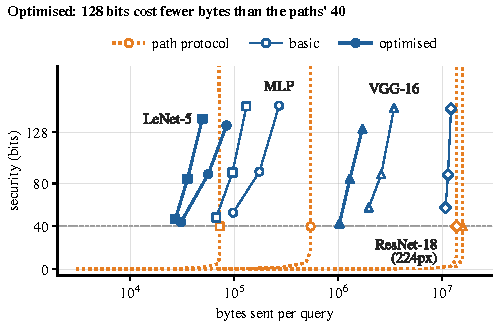
\includegraphics[width=\columnwidth]{figures/security_bits.pdf}
  \Description{Security bits against bytes sent per query for four image models: the path
  protocol with more and more paths, and our basic and optimised protocols at three security
  levels.}
  \caption{Security against bytes sent per query. The path protocol (dotted) reaches 40 bits only
  by opening the whole model and trace (vertical lines); the optimised protocol (filled) reaches
  128 bits with fewer bytes than that (hollow: basic; $\lambda = 40, 80, 128$).}
  \label{fig:security}
\end{figure}

Figure~\ref{fig:security} plots security against bytes. The basic protocol overshoots its target
because $r$ and $t$ are rounded up (48--58 bits at $\lambda{=}40$, 150--153 at $\lambda{=}128$),
and at $\lambda{=}40$ it sends 1.1--8.3$\times$ fewer bytes than the paths need for $2^{-40}$.
With the optimised protocol the achieved security lands closer to the target (43--47 and
131--141 bits), and on every model we ran it on, $2^{-128}$ costs fewer bytes than the paths need
for $2^{-40}$.

\subsection{Cost of the basic protocol}
\label{sec:cost}

\begin{table}[t]
  \caption{Image models: one query at $\lambda{=}128$, basic protocol. Proving takes milliseconds,
  and for the CIFAR models the proof is smaller than the int8 model.}
  \label{tab:cnn}
  \footnotesize
  \setlength{\tabcolsep}{2.6pt}
  \begin{tabular}{lrrrrrrr}
    \toprule
    & & & \multicolumn{3}{c}{committed ($\sC$)} & \multicolumn{2}{c}{$\Kpre$} \\
    \cmidrule(lr){4-6}\cmidrule(lr){7-8}
    Model & Params & int8 & prove & verify & proof & verify & proof \\
    \midrule
    MLP (MNIST) & 536K & 97.7\% & 3.1\,ms & 5.0\,ms & 270\,kB & 0.5\,ms & 3.1\,kB \\
LeNet-5 (MNIST) & 62K & 99.3\% & 4.3\,ms & 7.0\,ms & 131\,kB & 1.7\,ms & 26.1\,kB \\
VGG-11 (CIFAR) & 9.8M & 91.1\% & 14.7\,ms & 49.7\,ms & 2.2\,MB & 11.8\,ms & 610\,kB \\
VGG-16 (CIFAR) & 15.2M & 93.0\% & 21.5\,ms & 63.4\,ms & 3.4\,MB & 19.4\,ms & 1.1\,MB \\
ResNet-18 (CIFAR) & 11.2M & 94.2\% & 26.1\,ms & 110\,ms & 4.6\,MB & 46.5\,ms & 2.5\,MB \\
ResNet-18 (224px)$^\dagger$ & 11.2M & 95.0\% & 27.4\,ms & 175\,ms & 12.1\,MB & 105\,ms & 9.9\,MB \\
\bottomrule

  \end{tabular}

  \smallskip
  {\footnotesize $^\dagger$Our ImageNet-trained counterpart of the classifier of~\cite{anchuri2026verifiable}.}
\end{table}

\para{Image models.} With committed weights (Table~\ref{tab:cnn}) the prover needs 3.1--27\,ms per
query and the verifier 5.0--175\,ms. The proof, 131\,kB--12.1\,MB, is 2.4--4.4$\times$ smaller
than the int8 model for the VGGs and the CIFAR ResNet, and about its size for the 224-pixel ResNet,
whose claims grow with the number of pixels.

\begin{table}[t]
  \caption{Language models: next-token logits of one prompt at $\lambda{=}128$, basic protocol,
  random int8 weights (GPU: verifier on the GPU). Proving takes under 30\,s, and at 2{,}048 tokens
  the claims make up most of the proof.}
  \label{tab:llm}
  \footnotesize
  \setlength{\tabcolsep}{2.4pt}
  \begin{tabular}{lrrrrrrr}
    \toprule
    & & \multicolumn{4}{c}{committed weights ($\sC$)} & \multicolumn{2}{c}{$\Kpre$} \\
    \cmidrule(lr){3-6}\cmidrule(lr){7-8}
    Model & Params & prove & verify & GPU & proof & verify & proof \\
    \midrule
    \multicolumn{8}{l}{\emph{64-token prompts}} \\
    GPT-2 & 64 & 428\,ms & 924\,ms & 62.1\,MB & 280\,ms & 21.8\,MB \\
GPT-2 & 512 & 451\,ms & 1.7\,s & 213\,MB & 1.2\,s & 173\,MB \\
OPT-125M & 2{,}048 & 1.6\,s & 24.3\,s & 733\,MB & 22.2\,s & 692\,MB \\
OPT-1.3B & 2{,}048 & 11.0\,s & 1.9\,min & 3.8\,GB & 1.9\,min & 3.7\,GB \\
Qwen3-4B & 64 & 5.4\,s & 7.2\,s & 659\,MB & 2.2\,s & 284\,MB \\
OPT-6.7B & 2{,}048 & 32.5\,s & 3.4\,min & 10.1\,GB & 3.3\,min & 9.7\,GB \\
Llama-2-7B & 64 & 7.9\,s & 7.3\,s & 762\,MB & 2.2\,s & 349\,MB \\
Llama-2-7B & 2{,}048 & 35.6\,s & 3.7\,min & 11.6\,GB & 3.6\,min & 11.2\,GB \\
Llama-2-13B$^\ast$ & 64 & 14.0\,s & 13.2\,s & 1.2\,GB & 3.8\,s & 547\,MB \\
\bottomrule

  \end{tabular}
\end{table}

\para{Language models.} GPT-2 with a 64-token prompt is proved in 173\,ms and verified in 468\,ms
with a 62.1\,MB proof (Table~\ref{tab:llm}), and Llama-2-7B in 2.7\,s and 4.4\,s with a 762\,MB
proof, about 9$\times$ smaller than its int8 weights. At 2{,}048 tokens Llama-2-7B is still proved in
17.6\,s, but the proof grows to 11.6\,GB and CPU verification to 2.8\,min, because the verifier
recomputes attention over all token pairs; a GPU verifier is 21--41$\times$ faster there and
1.1--1.3$\times$ at 64 tokens. Committed weights make the prover of billion-parameter models
10--26$\times$ slower than known weights at up to 64 tokens, where opening the weights dominates,
and 1.0--1.8$\times$ at 2{,}048. Prompts whose claims are all sent before the challenge
can share one set of challenges and columns: in batches of eight 64-token prompts, Llama-2-7B
costs 0.40\,s and 401\,MB per prompt. For Llama-2-70B the extrapolated proof at 64 tokens is
3.7\,GB, 18$\times$ smaller than its int8 weights.

\begin{figure*}[t]
  \centering
  \begin{subfigure}[b]{0.32\textwidth}
    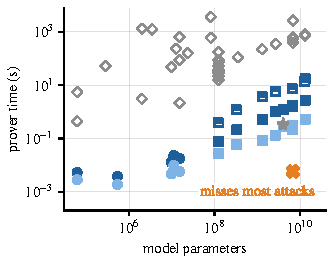
\includegraphics[width=\linewidth]{figures/cost_prover.pdf}
    \caption{Prover time}
    \label{fig:cost-prover}
  \end{subfigure}\hfill
  \begin{subfigure}[b]{0.32\textwidth}
    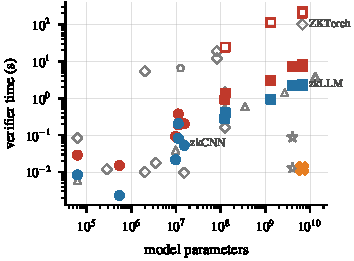
\includegraphics[width=\linewidth]{figures/cost_verifier.pdf}
    \caption{Verifier time (CPU, 8 threads)}
    \label{fig:cost-verifier}
  \end{subfigure}\hfill
  \begin{subfigure}[b]{0.32\textwidth}
    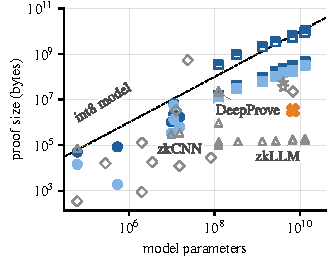
\includegraphics[width=\linewidth]{figures/cost_proof.pdf}
    \caption{Proof size}
    \label{fig:cost-proof}
  \end{subfigure}
  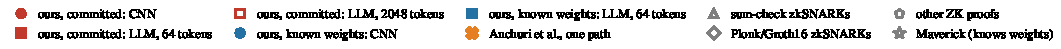
\includegraphics[width=\textwidth]{figures/cost_legend.pdf}
  \Description{Three log-log scatter plots of prover time, verifier time and proof size against
  model parameters, for our protocol and published systems.}
  \caption{Cost against model size (basic protocol; published systems as reported on their own
  hardware). Our prover is one to four orders of magnitude below the zkSNARK provers and our
  verifier is in their range, while our proof is usually larger and grows with the activations.}
  \label{fig:cost}
\end{figure*}

Figure~\ref{fig:cost} places these runs among the published ones. Part of the prover gap is our
GPU, since all the zkSNARKs except zkLLM ran on CPUs. The orange cross is one path
of~\cite{anchuri2026verifiable} as reported on an RTX~3090: cheap, but it catches the
single-neuron attack on Llama-2-7B with probability $1/11{,}008$.

\subsection{The optimised protocol}

\begin{table}[t]
  \caption{Basic $\to$ optimised protocol ($\sC$, interactive, $\lambda{=}128$ unless marked).
  In $\sC$ below 2{,}048 tokens the proof shrinks 2.0--4.2$\times$ and verification speeds up
  2.7--8.4$\times$.}
  \label{tab:opt}
  \footnotesize
  \setlength{\tabcolsep}{3pt}
  \begin{tabular}{lrrr}
    \toprule
    Model (tokens) & prove & verify & proof \\
    \midrule
    LeNet-5 (MNIST) & 4.3$\to$5.3\,ms & 7.0$\to$2.4\,ms & 131$\to$49.5\,kB \\
VGG-16 (CIFAR) & 21.5$\to$17.3\,ms & 63.4$\to$14.9\,ms & 3.4$\to$1.7\,MB \\
ResNet-18 (CIFAR) & 26.1$\to$20.6\,ms & 110$\to$24.7\,ms & 4.6$\to$2.3\,MB \\
GPT-2 (64) & 173$\to$80.2\,ms & 468$\to$92.0\,ms & 62.1$\to$14.8\,MB \\
GPT-2 (512) & 163$\to$134\,ms & 1{,}012$\to$375\,ms & 213$\to$89.5\,MB \\
Llama-2-7B (1) & 2.7$\to$1.5\,s & 2{,}527$\to$299\,ms & 418$\to$130\,MB \\
Llama-2-7B (64) & 2.7$\to$1.7\,s & 4.4$\to$1.1\,s & 762$\to$329\,MB \\
Llama-2-7B (2{,}048)$^g$ & 17.6$\to$\pending{17.6}\,s & 6.9$\to$\pending{6.9}\,s & 11.6$\to$\pending{11.6}\,GB \\
Qwen3-4B (8)$^k$ & 135$\to$119\,ms & 263$\to$156\,ms & 36.1$\to$20.3\,MB \\
\bottomrule

  \end{tabular}

  \smallskip
  {\footnotesize Optimised: planning rule and compact encoding; GPT-2 and Qwen3-4B also compute the
  last block at the last position only. $^g$GPU verifier, streaming when optimised; proof
  unchanged. $^k\Kpre$, $\lambda{=}40$, one verifier thread, embedding look-ups.}
\end{table}

We re-ran the image models other than the 224-pixel ResNet, GPT-2 at 64 and 512 tokens,
Llama-2-7B at 1 and 64 tokens, Qwen3-4B in Maverick's setting and five of zkLLM's models at
2{,}048 tokens with the optimisations, on the same machines. All 4{,}380 honest queries were
accepted and all 4{,}973 attacks rejected, 3{,}300 of them on image models under the planning
rule. With committed weights, for images and prompts of up to 512 tokens, the proof
becomes 2.0--4.2$\times$ smaller and verification 2.7--8.4$\times$ faster (Table~\ref{tab:opt}).
Much of the verifier's gain comes from the verifier engineering alone, which also speeds up the
basic proofs (468 to 197\,ms for GPT-2 at 64 tokens). At 2{,}048 tokens the claims are about 95\%
of the proof, which keeps its size, but Llama-2-7B is proved in 5.4\,s instead of 18.7\,s and
verified in 1.7\,s instead of 6.9\,s. Both gains come from the int32 attention, which the prover
shares with the verifier, and from the streaming verifier; we did not separate the two. The
committed-weights prover then takes 1.9$\times$ the plain int8 forward pass. In exchange the
one-time setup is longer (114--198\,s instead of 10--11\,s for GPT-2, about 8.5 instead of 4.5\,min for
Llama-2-7B), and one cell regressed. For Llama-2-13B in setting $\sC$ the streaming verifier takes
9.1\,s, 5.4$\times$ Llama-2-7B's, and host memory peaks at 63\,GiB, for reasons we have not
found.

\subsection{Comparison with published systems}
\label{sec:compare}

\begin{table}[t]
  \caption{Optimised protocol against published systems on matched models (theirs/ours;
  $\uparrow$: ours better; bold: better on all three; ours prove the next-token logits). Our prover
  is faster everywhere; our proof is smaller only in the bold rows and against Maverick.}
  \label{tab:ratios}
  \footnotesize
  \setlength{\tabcolsep}{3.5pt}
  \begin{tabular}{llrrr}
    \toprule
    System & Model (tokens) & prover & verifier & proof \\
    \midrule
    zkCNN & LeNet-5 & 103$\times$$\uparrow$ & 1.2$\times$$\downarrow$ & 1.8$\times$$\downarrow$ \\
Bionetta & LeNet-5 & 878$\times$$\uparrow$ & 1.4$\times$$\uparrow$ & 149$\times$$\downarrow$ \\
zkCNN & VGG-16 & 4{,}108$\times$$\uparrow$ & 1.1$\times$$\downarrow$ & 10$\times$$\downarrow$ \\
ZKML & VGG-16 & 29{,}644$\times$$\uparrow$ & 6.6$\times$$\downarrow$ & 285$\times$$\downarrow$ \\
zkGPT & GPT-2 (64) & 126$\times$$\uparrow$ & 1.3$\times$$\downarrow$ & 615$\times$$\downarrow$ \\
DeepProve & GPT-2 (64) & 198$\times$$\uparrow$ & 2.9$\times$$\uparrow$ & 2.9$\times$$\downarrow$ \\
DeepProve & GPT-2 (512) & 1{,}082$\times$$\uparrow$ & 1.6$\times$$\uparrow$ & 8.4$\times$$\downarrow$ \\
zkLLM & OPT-125M (2{,}048) & 70$\times$$\uparrow$ & 42$\times$$\downarrow$ & 5{,}195$\times$$\downarrow$ \\
zkLLM & OPT-350M (2{,}048) & 36$\times$$\uparrow$ & 65$\times$$\downarrow$ & 13{,}309$\times$$\downarrow$ \\
zkLLM & OPT-1.3B (2{,}048) & 39$\times$$\uparrow$ & 88$\times$$\downarrow$ & 25{,}898$\times$$\downarrow$ \\
zkLLM & OPT-2.7B (2{,}048) & 34$\times$$\uparrow$ & 93$\times$$\downarrow$ & 41{,}577$\times$$\downarrow$ \\
zkLLM & OPT-6.7B (2{,}048) & 34$\times$$\uparrow$ & 78$\times$$\downarrow$ & 64{,}338$\times$$\downarrow$ \\
zkLLM & OPT-13B (2{,}048) & 29$\times$$\uparrow$ & 54$\times$$\downarrow$ & 98{,}447$\times$$\downarrow$ \\
zkLLM & Llama-2-7B (2{,}048) & 35$\times$$\uparrow$ & 72$\times$$\downarrow$ & 63{,}313$\times$$\downarrow$ \\
zkLLM & Llama-2-13B (2{,}048) & 30$\times$$\uparrow$ & 57$\times$$\downarrow$ & 96{,}436$\times$$\downarrow$ \\
ZKTorch & Llama-2-7B (1) & 974$\times$$\uparrow$ & 40$\times$$\uparrow$ & 18$\times$$\downarrow$ \\
Maverick & Qwen3-4B (8) & 2.6$\times$$\uparrow$ & 3.0$\times$$\downarrow$ & same \\
\bottomrule

  \end{tabular}

  \smallskip
  {\footnotesize $^a$Interactive (Fiat--Shamir not run). $^b\Kpre$, $\lambda{=}40$, one client
  thread; Maverick's time includes its non-linear replay. $^c$zkLLM's public code on our L40S.}
\end{table}

Table~\ref{tab:ratios} compares the optimised protocol with published systems, each in the
matching setting: Fiat--Shamir against non-interactive systems, the interactive protocol against
zkLLM and Maverick, which are interactive themselves, and committed weights except against
Maverick, whose client knows the weights. Our verifier uses 8 CPU threads (one against Maverick,
like its client), or the GPU at 2{,}048 tokens. Prompt lengths match, except that zkGPT states
none and we use 64 tokens.

\para{Prover.} Ours is faster than every zkSNARK prover on its matched model, by 53$\times$
(zkLLM, Llama-2-13B) to 32{,}000$\times$ (ZKML, VGG-16). Part of this is hardware, so we also ran
zkLLM's public code on our L40S. Its demo proves the components of one layer separately and
reports no verifier time, so we time one layer (median of three runs on each of two layers) and
multiply by the number of layers. The demo lacks zkLLM's cross-layer optimisation and the attention
output projection, and its attention step writes no output, so we count a layer's second skip
connection twice. For Llama-2-7B at
2{,}048 tokens this gives about 844\,s, 157$\times$ our 5.4\,s (48$\times$ the basic protocol's
17.6\,s). We do not use the demo for Llama-2-13B, whose time per layer grows out of proportion
(2.5$\times$ the 7B figure).

\para{Verifier and proof.} Our verifier is faster than all but three, ZKML's on VGG-16
(1.9$\times$), zkLLM's on Llama-2-13B (2.3$\times$) and Maverick's (1.2$\times$). Maverick's
time, 124.5\,ms, is its 87.1\,ms of matrix checks plus the 37.4\,ms in which its client replays the
non-linear operations, work that our verifier also does; ours takes 155.5\,ms. On LeNet-5 and on
GPT-2 with a 64-token prompt the optimised protocol wins on all three costs: 5.4\,ms, 2.6\,ms and 63.3\,kB against zkCNN's 441\,ms, 5.8\,ms and 71.3\,kB,
and 91\,ms, 105\,ms and 16.6\,MB against DeepProve's 34.2\,s, 1.35\,s and 21.7\,MB. Both wins come
with caveats. zkCNN's verifier ran on one core and ours on eight threads, and zkCNN's protocol has
a zero-knowledge variant, which ours lacks. DeepProve's figures are for its transparent (BaseFold)
configuration, whose proof certifies every position of its 64-token sequence where ours certifies
the next-token logits; its HyperKZG configuration, which needs a structured reference string,
sends 9.4\,MB. Elsewhere the proof is our cost, 3.6--180$\times$ larger than the other
short-input proofs and 5{,}200--96{,}000$\times$ larger than zkLLM's at 2{,}048 tokens. In
Maverick's own setting our proof is 1.8$\times$ smaller and our prover, on the GPU, 3.0$\times$
faster than its 64-thread CPU prover, but Maverick draws a fresh challenge per query, whereas
$\Kpre$ reuses a secret one.

% =====================================================================================
\section{Discussion}

\para{What this means.} Sampling-based proofs of inference are sound only against a weak
adversary: they catch a provider who honestly runs the wrong model, but not one who runs the
committed model and edits the answer. None of the sampling rules we analysed closes that gap at
sub-linear cost. Full soundness does not require a zkSNARK's prover cost. One random linear
combination per weight layer gives a $2^{-\lambda}$ guarantee with no trusted setup and no
assumption about how models behave. The client it
suits is a gateway or an auditor with a GPU and a fast link rather than a phone, because at long
prompts the verifier still recomputes attention. Large models with short prompts suit it best,
since there the optimised proof is far smaller than the model (21$\times$ for Llama-2-7B at 64
tokens).

\para{Limitations.} (i)~The proof grows with the activations; at 2{,}048 tokens it is about 95\%
claims and gigabytes for 7B models, against zkLLM's 157--183\,kB. (ii)~The verifier's cost grows with the
square of the prompt length: at 2{,}048 tokens the CPU verifier needs minutes, and on a GPU the
optimised verifier beats zkLLM's on four of five models but is 2.3$\times$ slower on Llama-2-13B. (iii)~The provider
must serve the integer model, which changed CNN accuracy by at most 0.4 points and raised the
perplexity of real OPT checkpoints by 7--33\% (constants chosen on the evaluation text); the LLM
costs were measured with random weights. (iv)~Like the path protocol we assume an honest weight
commitment, which the optimised codes make up to 19$\times$ slower to compute; a malformed one would
need a proximity argument as in Ligero. (v)~The opened columns reveal random linear combinations
of each weight row, so the protocol is not zero-knowledge. (vi)~We prove one forward pass, without
a KV cache. (vii)~The prototype is Python, and the same-GPU zkLLM comparison rests on its demo.

\para{Future work.} The claims, which the compact encoding only halves, could be replaced by a
sum-check argument for the non-weight operations; a native verifier and a KV cache would also
help, and per-channel normalisation gains may narrow the perplexity gap at no proving cost. Before
any wider publication we will share the attack with the authors of~\cite{anchuri2026verifiable}.

% =====================================================================================
\section{Conclusion}
A single tampered neuron defeats the lightweight path-sampling proof of inference
of~\cite{anchuri2026verifiable}, on an MNIST network and on the real OPT-6.7B, and no sampling
rule we analysed repairs it at sub-linear cost. Checking every layer with Freivalds' algorithm
against a Reed--Solomon/Merkle commitment does: our verifier accepts a wrong output with
probability at most $2^{-\lambda}$ and rejected all 2{,}895 attacks, our prover is one to four
orders of magnitude faster than published zkSNARK provers, and the optimised protocol also beats
zkCNN on LeNet-5 and DeepProve's transparent configuration on GPT-2 in verifier time and proof
size. Long prompts, where the proof is mostly claims, remain its weak point.

% =====================================================================================
\section{Contributions}
% TODO (team): replace with the actual split of work before submitting.
\textcolor{red}{[To be completed by the team.]} Ofek Lavi: \textcolor{red}{[\dots]}.
Erel Barzilay: \textcolor{red}{[\dots]}. Edo Kadosh: \textcolor{red}{[\dots]}.

\bibliographystyle{ACM-Reference-Format}
\bibliography{references}

\end{document}
